\section{Analysis Results}
In this section, we describe the application of our system, \sysname on real world to gather information on the working of service workers and it's role in notification service. We calculate measurements that help us understand the advertising ecology and their behaviour. We use the filtered URLs that requested for notification permission and monitor these URLs as mentioned in \ref{monitoring}. We have collected data over multiple periods of time while making any improvements that are required to the system based on the data observed previously. 

\subsection{Notifications in the Wild}
From the logs collected over a initial set of URLs, we were able to obtain the time taken by websites to request for notification permission and it is shown in fig.\ref{req_time}. We could observe from this figure that over 95 percent of the websites took under 3 minutes to request notification. Hence, of the 3000 websites that were used for this measurement, 2850 websites requested permission under 3 minutes. This helped us to decide on the wait time of 5 minutes for which we keep a website open on the browser while visiting the website for the first time. The 5 minutes wait time also takes into consideration any delay caused in loading the website. 

\begin{figure}[h]
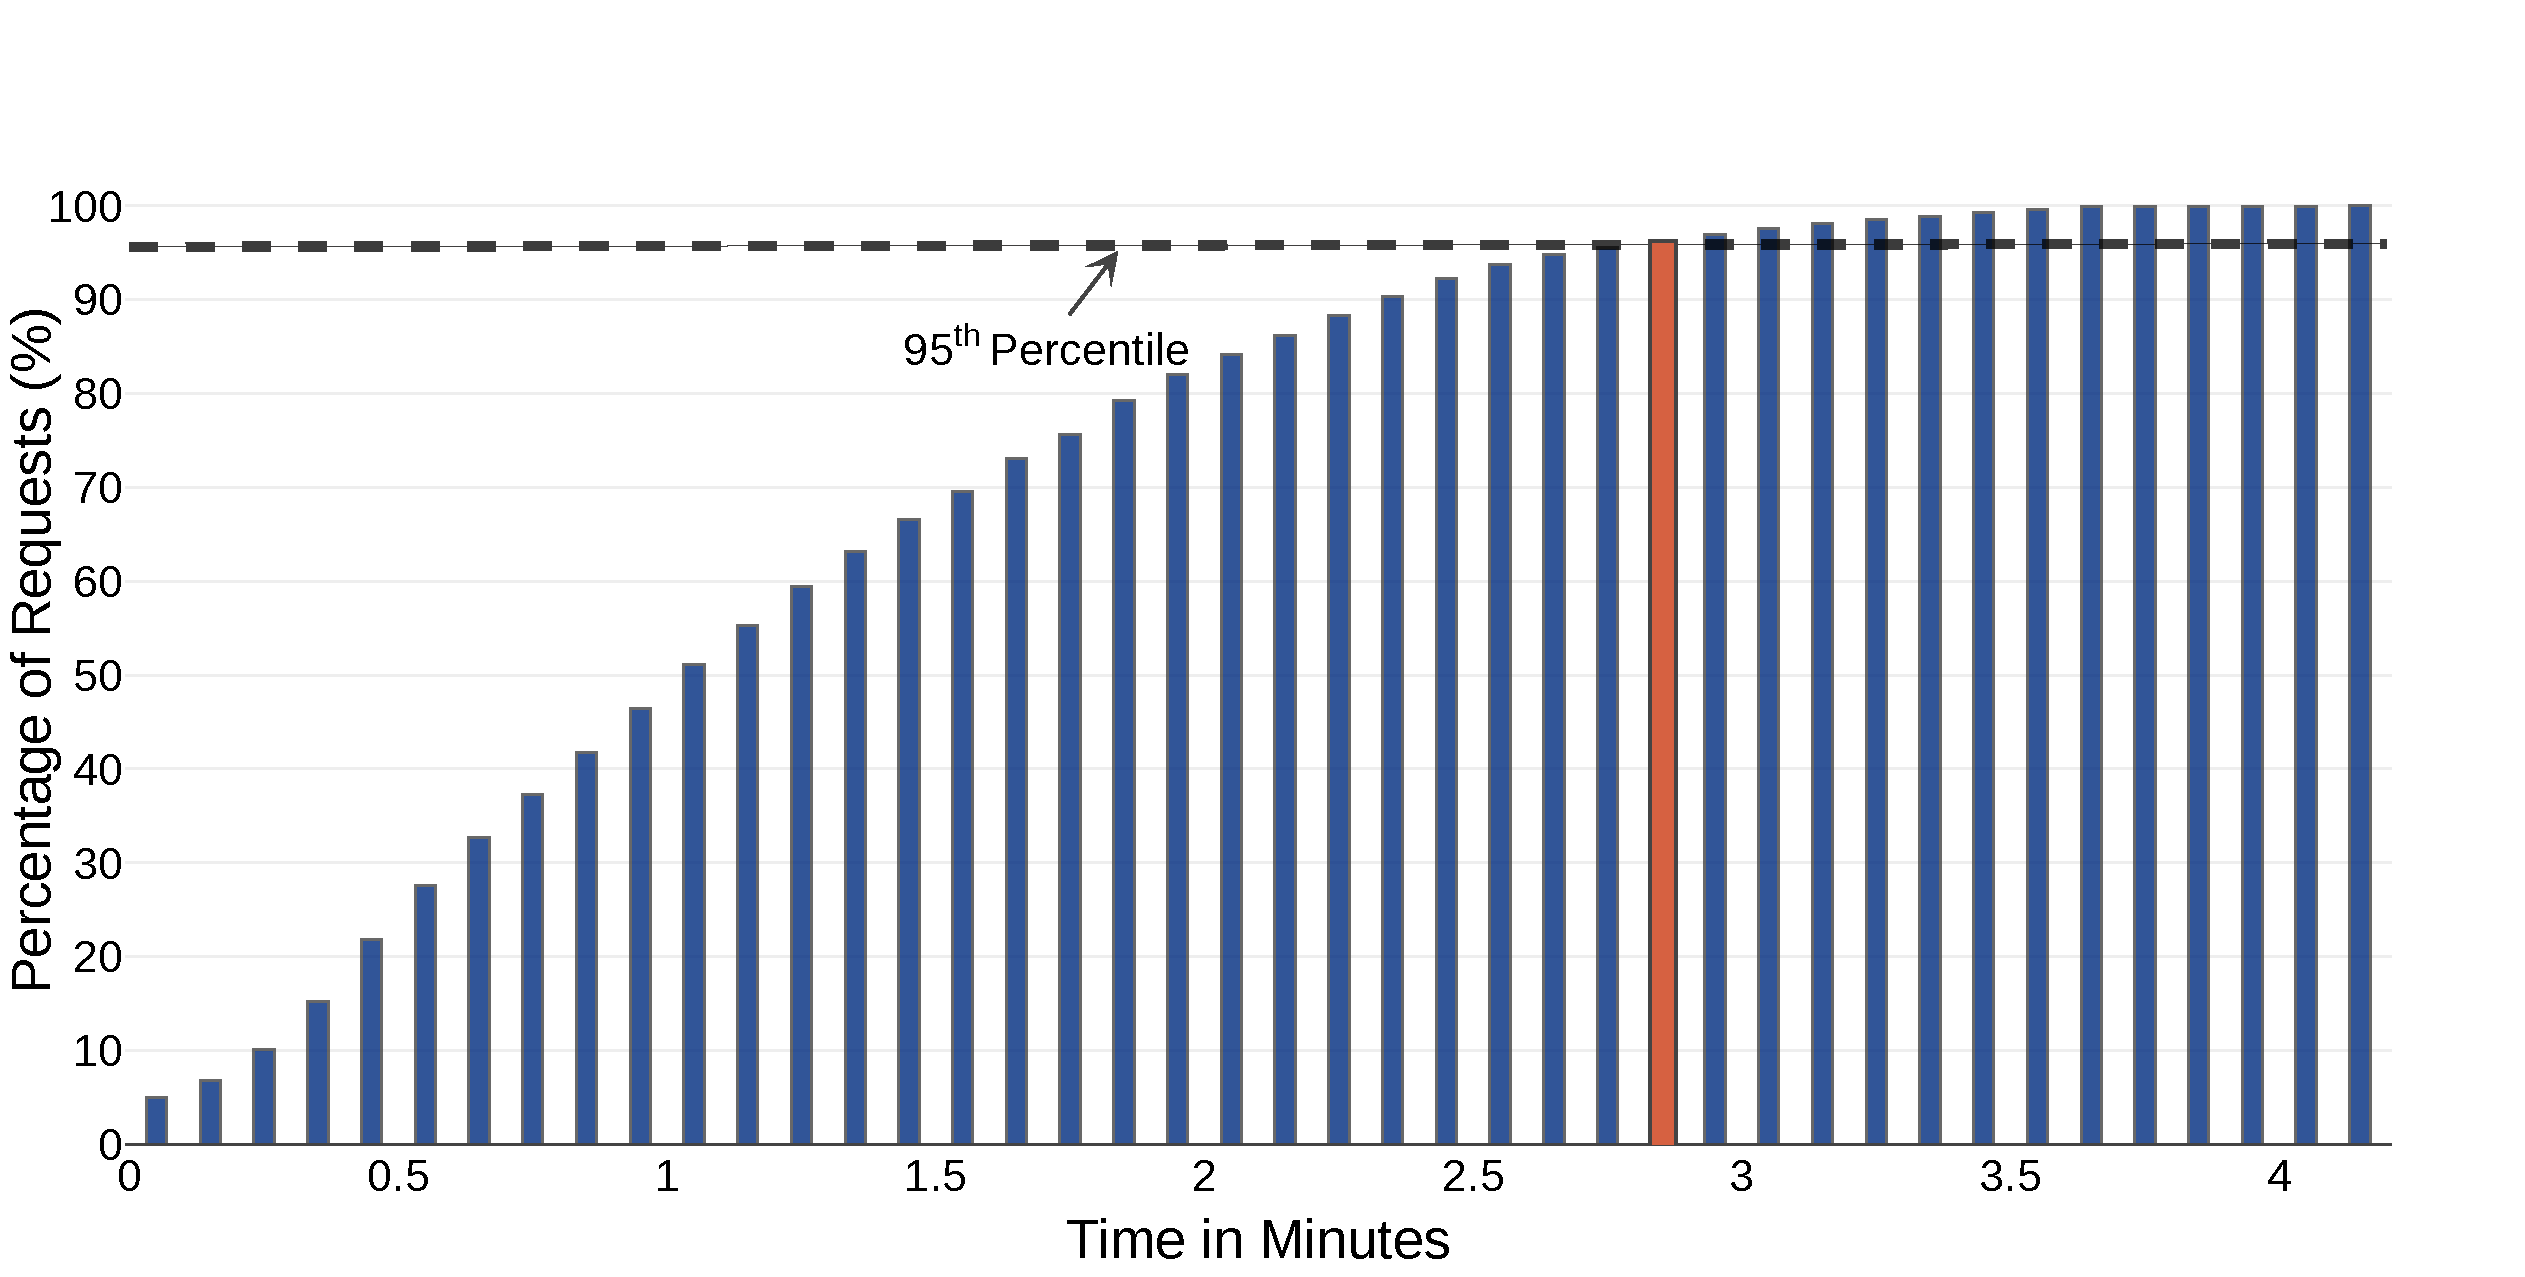
\includegraphics[width=\columnwidth]{figs/req_time.pdf}
\caption{CDF of time taken by sites to request permission. The number of requests made by websites are shown in percentage in y axis. }
\label{req_time}
\end{figure}

Next, We obtain the time it takes for a website to send it's first notification and we collect this measure from multiple websites that we monitored and the result is shown in fig.(\samuel{There's a string macro called \figurename. You might want to use that?}) \ref{first_notification}. This measure helped us decide the duration for which a docker session in desktop environment should be kept active. Next, we measure the count of notifications sent by a website to the end user per day. The results are quite alarming and a vast difference between mobile and desktop environment can be observed. We count the number of notifications sent by a service worker per day and calculate minimum, maximum and average number of notifications over multiple days and plot them in a graph as portrayed in fig. \ref{notification_per_day}. We had 506 and 303 service workers from desktop environment and mobile environment respectively. The maximum number of notifications sent by a service worker turned out to be \textbf{90} and \textbf{316} for desktop and mobile respectively. Around 12\% and 20\% of the service workers have sent over 10 notifications on an average per day in desktop and mobile environment respectively. It can be observed from these numbers that mobile users are targeted and preferred more by malicious ad networks.

\begin{figure}[h]
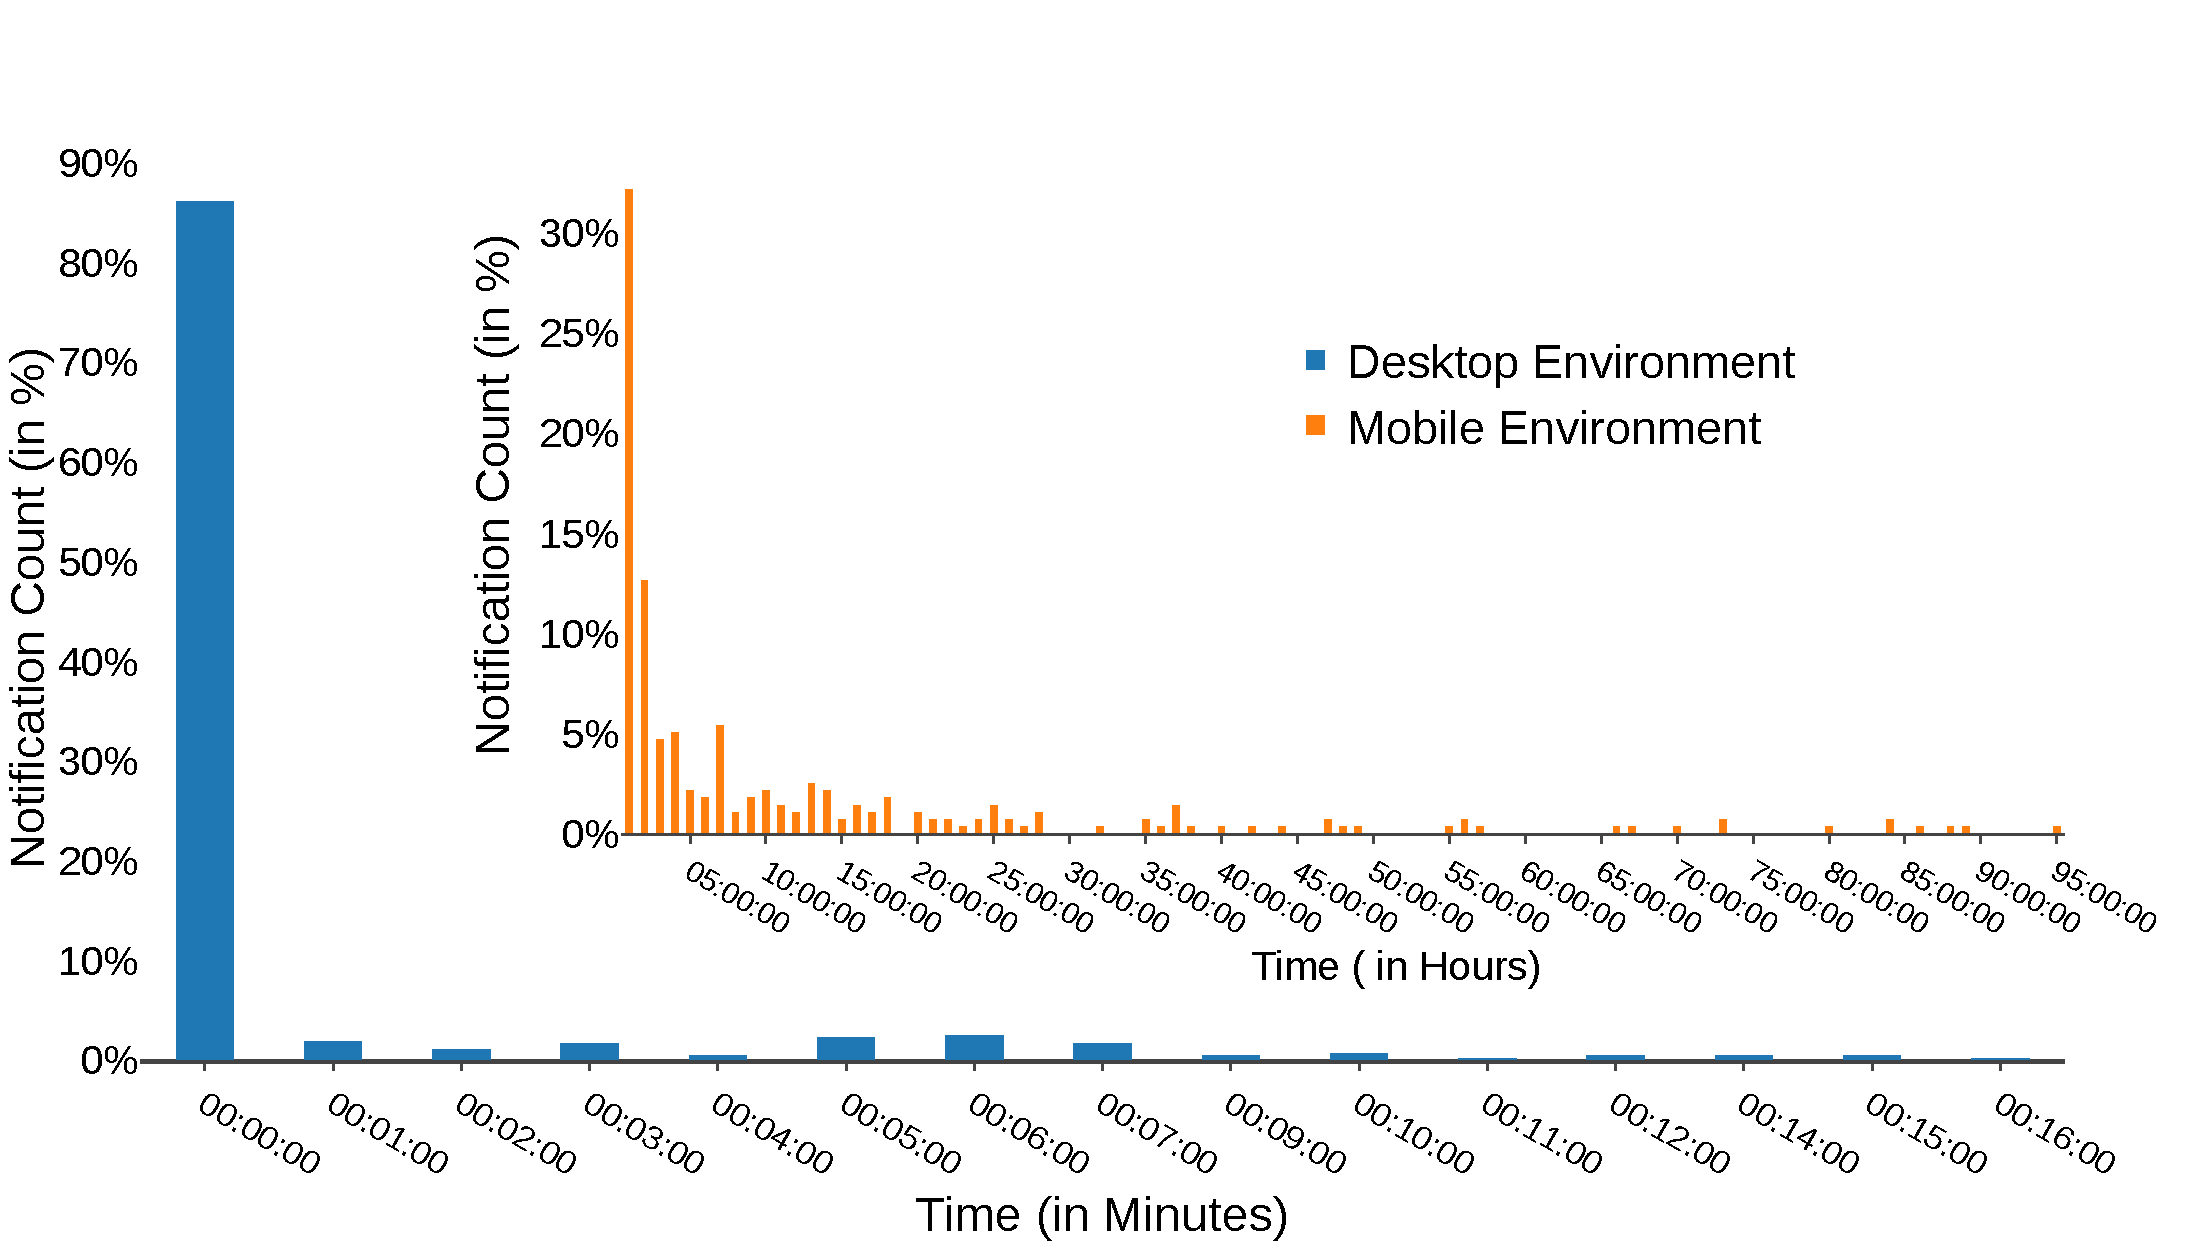
\includegraphics[width=\columnwidth]{figs/first_notification_histo.pdf}
\caption{Time taken for websites to send their first notification}
\label{first_notification}
\end{figure}

% \begin{figure}[h]
% 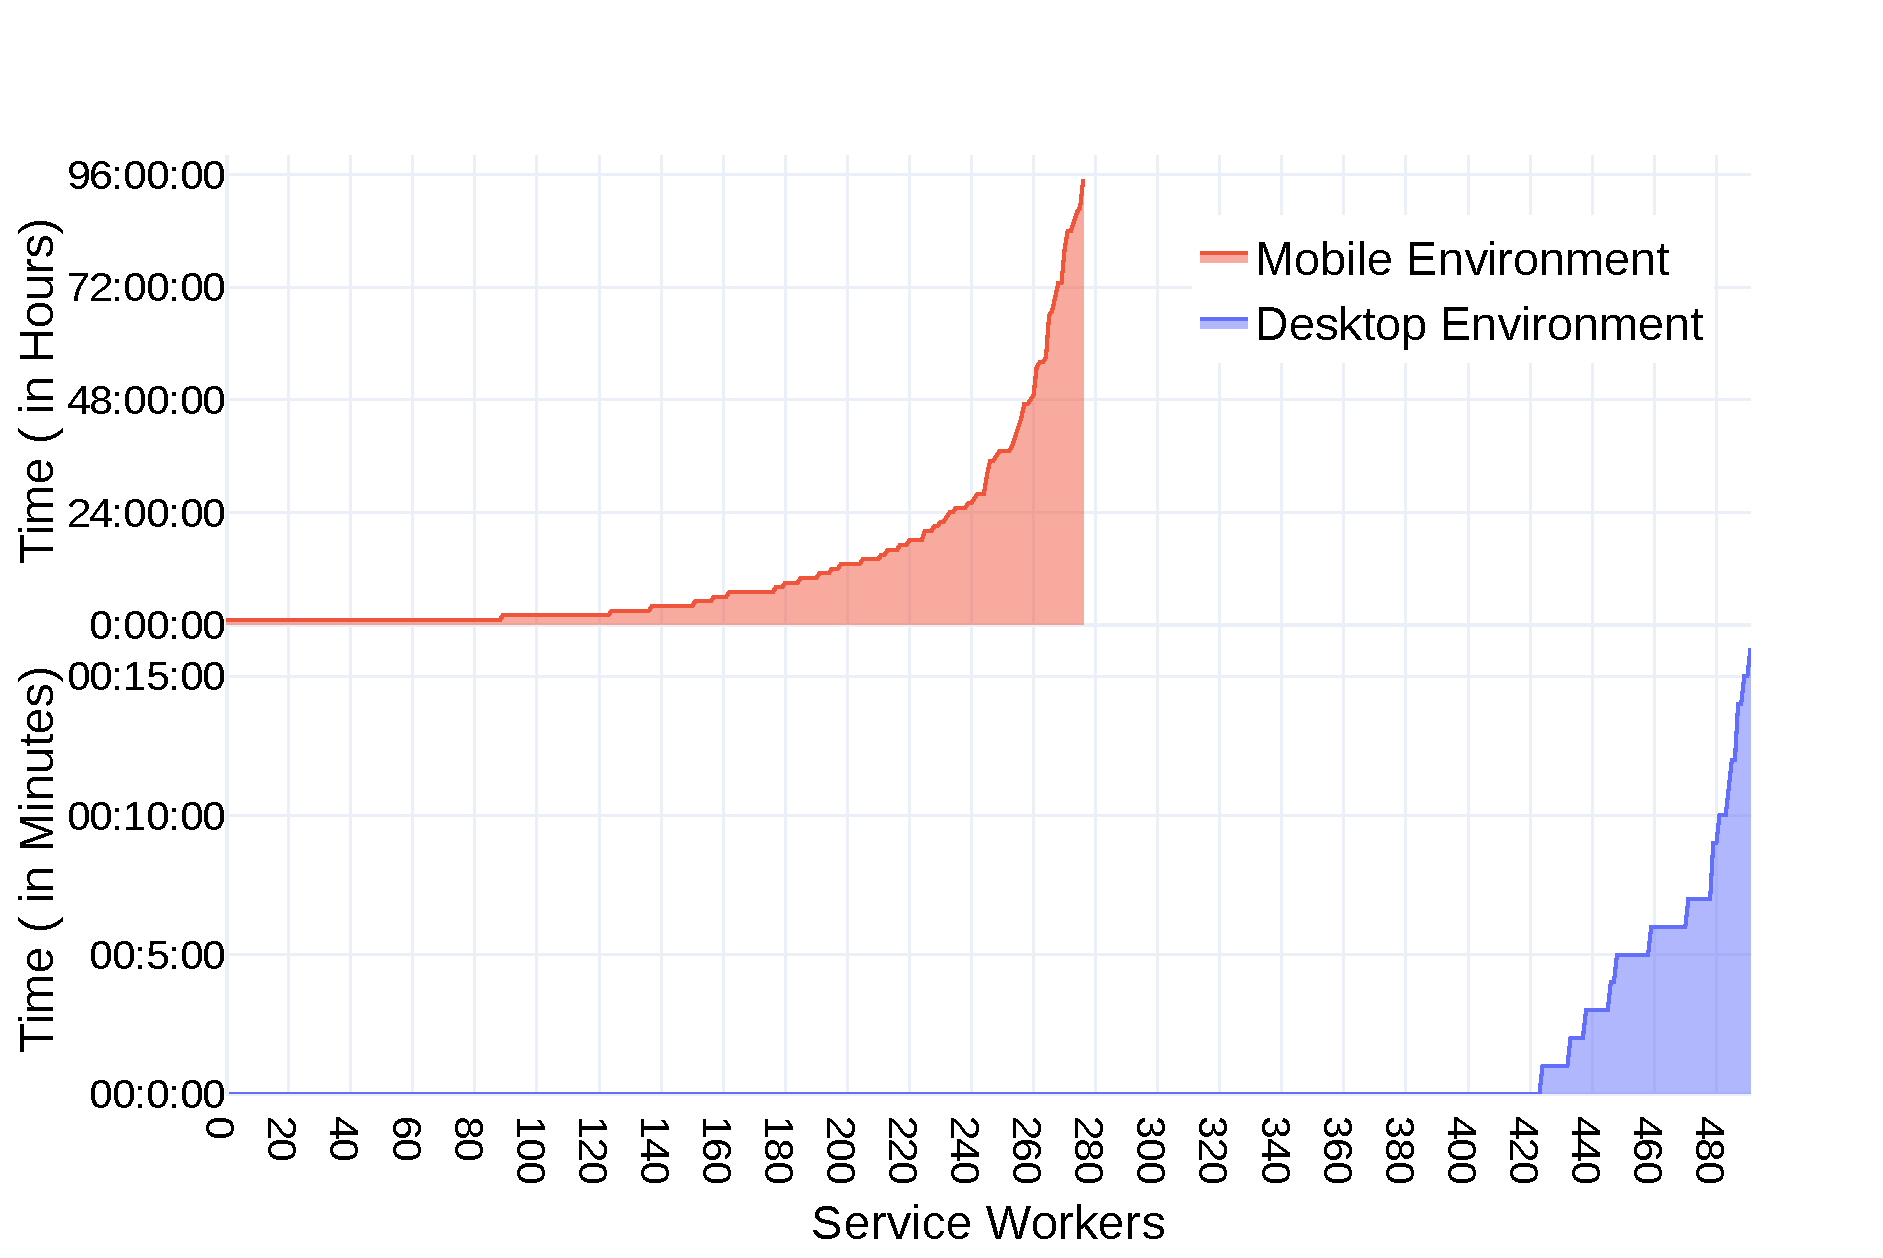
\includegraphics[width=\columnwidth]{figs/first_notifications.pdf}
% \caption{Time taken for websites to send their first notification}
% \label{first_notification}
% \end{figure}


% \begin{figure}[h]
% 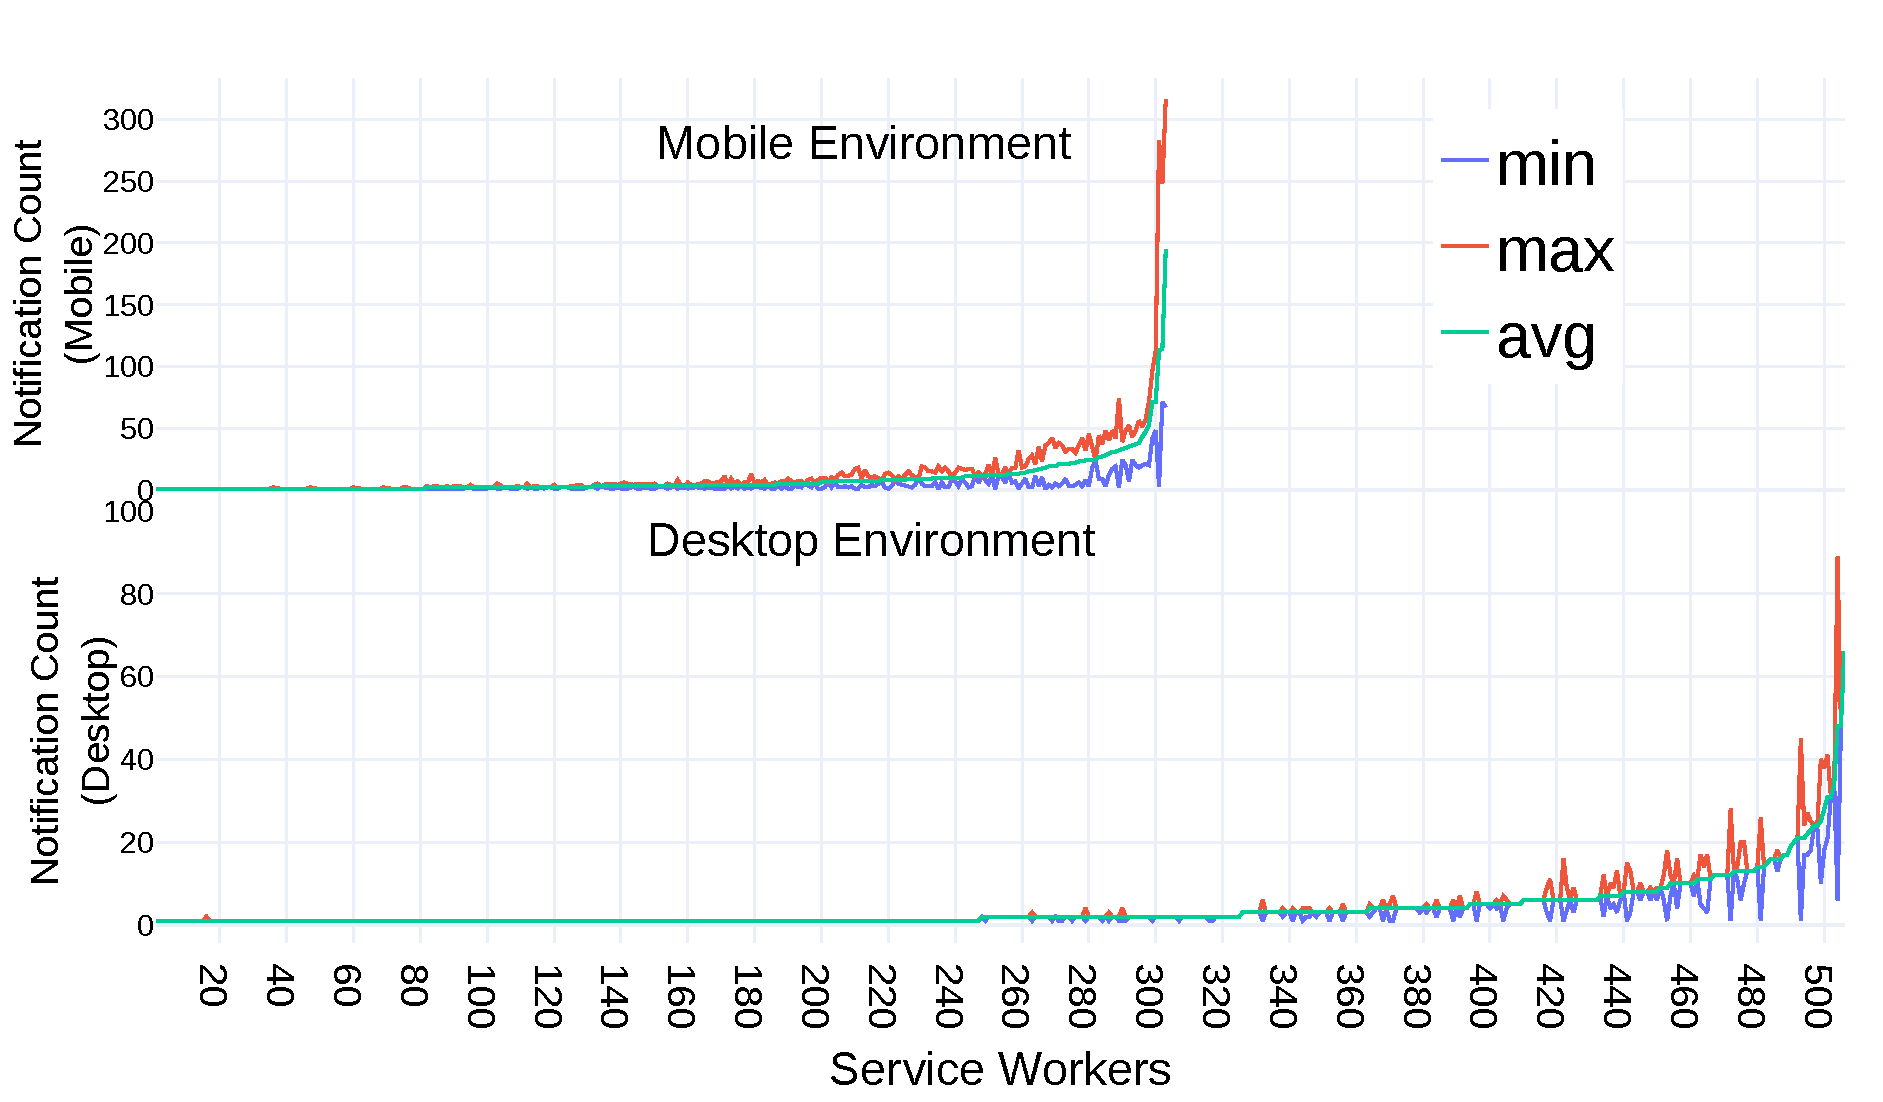
\includegraphics[width=\columnwidth]{figs/avg_not_dm.pdf}
% \caption{Number of notifications per day}
% \label{notification_per_day}
% \end{figure}

\begin{figure}[h]
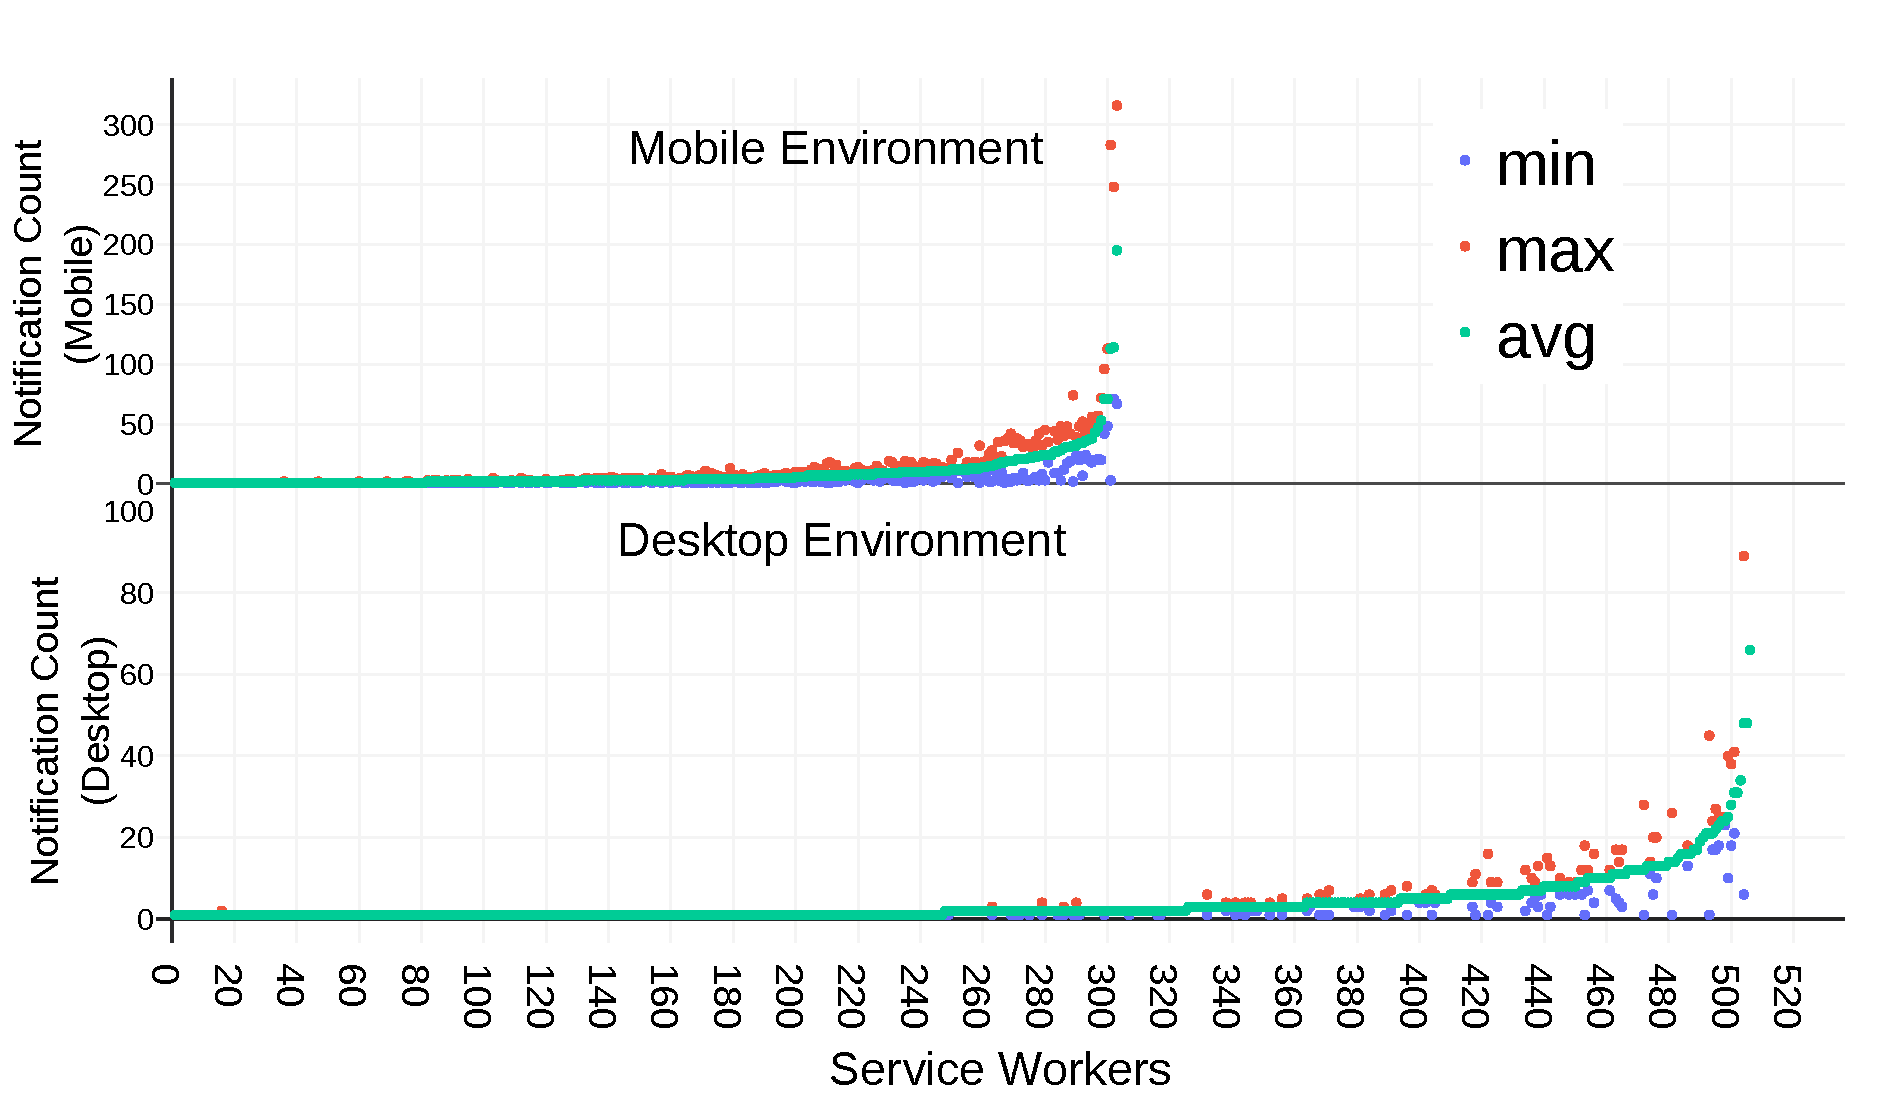
\includegraphics[width=\columnwidth]{figs/avg_notifications.pdf}
\caption{Number of notifications per day}
\label{notification_per_day}
\end{figure}

\subsection{Advertisements, their properties and patterns}
In this section, we explain in detail how we identify various ad campaigns, ad networks responsible for the campaigns and determine the maliciousness of the ads. At the end of our data collection stage, we had logged over 5000 and 3000 notifications in desktop and mobile environment. Over 20\% of notifications collected belong to languages other than English. We make use of Google Translate's online service to translate as many notifications as possible to English. The different information we found useful for the next stages of analysis are notification title, notification body, service worker file , landing URL, website's trust score, landing domain's trust score, IP address and WHOIS information of landing domain and the first domain contacted by the service worker and the data from Google safe browsing list and Virus total blacklists. Due to large amount of data and it's information, we perform a layered clustering of data. At each layer of clustering, we consider different sets of information that would identify the patterns if any among the ads and ad networks. The multiple layers are explained in the following sections

\subsubsection{Discovering Ad Campaigns}
Ad campaigns are defined as set of advertisements that delivers a similar message and are created with a particular goal. From a security perspective, we consider ad campaigns to be the set of ads that follow similar pattern with their main goal as 'to attract as many user clicks' as possible. To obtain advertisements with similar message/pattern, we consider the features notification title and notification body. We use the combined text of both features and clean them for stop words, convert any smileys into their word representations using \ref{simley_to_text} and vectorize the data. We use \texttt{gensim.similarities.SoftCosineSimilarity} to calculate the similarity between the samples. We chose soft cosine similarity measure over Jaccard and Cosine similarity measure as the former is known to identify the slightest common patterns between two given sentences compared to the latter ones \ref{soft_cosine}. Then, we perform an Agglomerative Hierarchical clustering on the distance matrix calculated from the soft cosine similarity matrix. We performed agglomerative clustering for various clusters based on the dendogram as shown in fig \ref{dendogram}. We then manually analyzed the results for few cut-offs to determine the best cut-off as 0.7 for which the clusters had relevant samples.Some examples of these clusters are shown in Fig.\ref{text_cluster}.  At this cut-off, the algorithm clustered 2700 samples into 750 clusters. 

%% change explanation using silhoutte score for the clusters

\begin{figure}[ht]
\caption{Examples of Ad Campaigns }
\begin{center}
\label{text_cluster}
\begin{tabular}{c}
\hline


 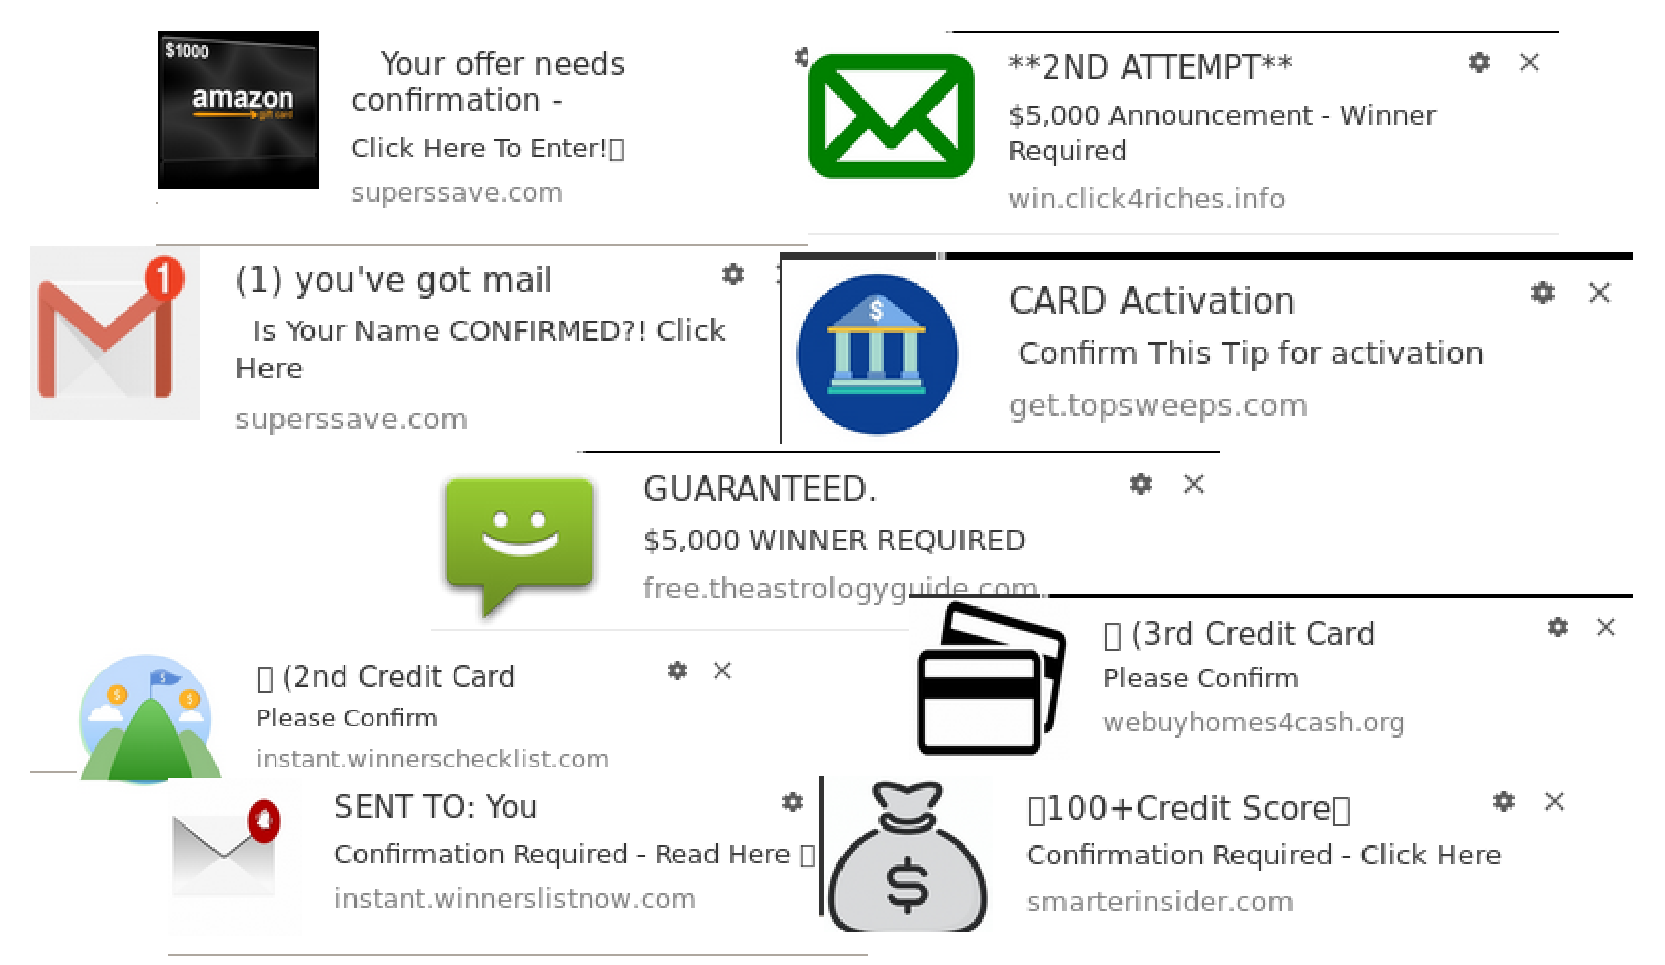
\includegraphics[scale=0.28]{figs/notifications.pdf}{C1}

\\
\hline
\hline

 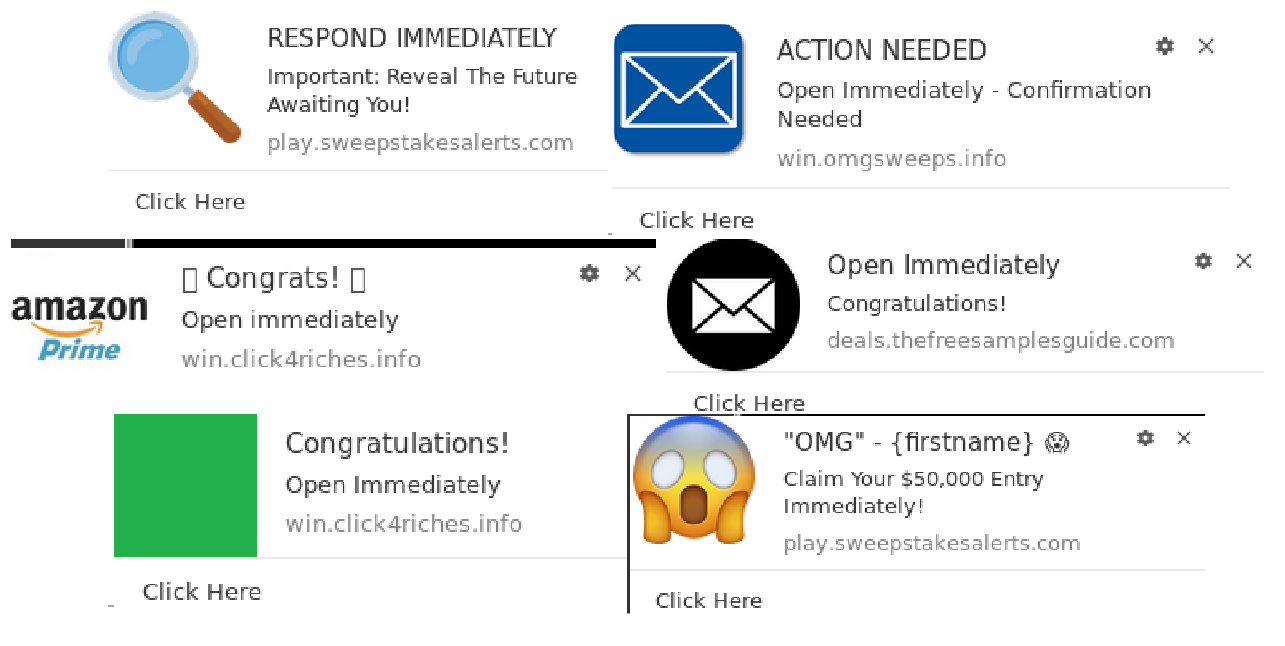
\includegraphics[scale=0.28]{figs/notifications2.pdf}{C2}

 \\
 \hline
    \end{tabular}
\label{tab1}
\end{center}
\end{figure}


\subsubsection{Topic Detection on Clustered Advertisements}
Looking over the clusters manually, we found a lot contextual similarity between the ads that belonged to a cluster and across clusters. To obtain a higher sense of the topics each clusters dealt with, we performed a topic modelling on the clusters using LIWC dictionary \ref{LIWC}. AS each advertisement has fewer number of words, we merge the samples that belong to each clusters and provide it as input to the topic modeller. From the topics listed by LIWC dictionary, we removed the topics related to linguistics and was left with 32 topics. The Fig. \ref{topic_cloud} illustrates the distribution of these topics among the ad clusters. We use these topics discovered for each ad cluster in next stage of clustering. The word cloud tells us that most of the advertisements we gathered had tried to attract users by trying to reward them with money or gifts. On the contrary, we also found a number of notifications focused on scaring the users into clicking ads regarding their bank accounts, health issues and mails.

\begin{figure}[ht]
\begin{center}
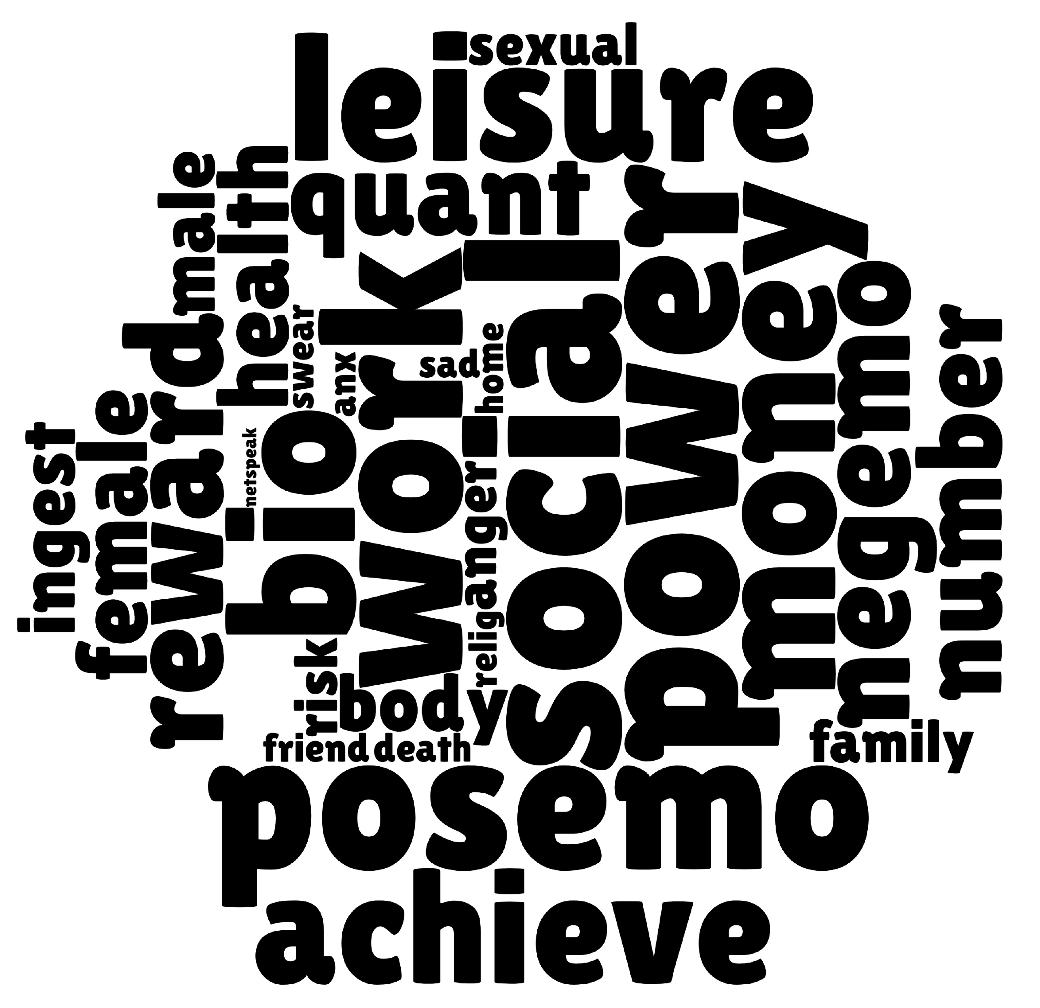
\includegraphics[ scale=0.4]{figs/topic_cloud.pdf}
\caption{Word Cloud on Topics detected in collected ads }
\label{topic_cloud}
\end{center}
\end{figure}


\subsubsection{Discovering Similar Behaviour in Advertisements and Ad Networks}
This is the third and final layer of clustering. At this stage, we use the features mentioned in table \ref{features} to cluster the advertisements. This clustering brings together advertisements that lead to same URL or IP address or location; belong to same ad network; deal with similar topics. To achieve this, we used K-means clustering with 3000 advertisements as input and obtained 250 clusters.

\begin{table}[htbp]
\caption{Features }
\begin{center}
\label{features}
\begin{tabular}{p{2.5cm}|p{5.5cm}}
\toprule
\hline
 \textbf{Features} & \textbf{Explanation}
 \\
 \hline
 Ad Campaign Ids & Output from First stage of clustering on notification title and body 
 \\
  \hline
 Ad Topics & Topics obtained from detection  using LIWC dictionary
 \\
 \hline
 Ad Network Domain & First Domain that the service worker contacted after registration
 \\
  \hline
 IP address & IP address of the final URL the advertisement leads user to 
 \\
 \hline
 Landing Domain & Domain name of the final URL the advertisement leads user to 
 \\
 \hline
 Latitude & Latitude of the landing URL's IP
\\
\hline
 Longitude & Longitude of the landing URL's IP
\\
 \hline
 WHOIS name & Party responsible for registering the landing domain
 \\
 \hline
 \bottomrule
\end{tabular}
\end{center}
\end{table}

\noindent \textbf{Categorizing Push Advertisements}
During the analysis of clusters, we categorize advertisements based on the content of their landing page. Different categories that we came across in our samples and the number of URLS for each cases are shown in \ref{categories}. Since visiting each page to determine it's category involves a lot of manual effort, we only visit a subset of our data samples. For example, We don't try and visit those cases that are in languages other than English as we might not fully understand it's content and hence fail in categorizing them. On analyzing these chosen samples, we found certain ads and the landing pages to be suspicious. We consider suspicious advertisements to be the ads that lead user to known malicious pages or to pages that appear to be phishing or scam pages built to deceive users or to pages that are irrelevant to the advertisement's context. We use multiple parameters to determine if an advertisement is suspicious in nature. 

\begin{itemize}
    \item To identify known malicious domains and pages, we check the URLs that we come across during our experiments on Google Safe Browsing(GSB) and Virus Total reporting tool.
    \item Next, We submit the URLs on Virus Total's scanning platform. This platform scans the submitted URLs in the background and update the results about their maliciousness. This identifies malicious pages that are not blacklisted until we submitted them as suspicious URLs.
    \item If a sample in a cluster is found to be malicious, we suspect other members of the cluster and perform detailed analysis on those samples
    \item We consider same ads leading to multiple landing pages within a single cluster as suspicious.
    \item If there are multiple landing domains/ URLs following the same naming/URL pattern, we tag them suspicious for further manual verification.
\end{itemize}
   
To our surprise, we found that the most popular blacklists available such as GSB and Virus Total were unaware of lot of URLs that we scanned with them. When we submit the URLs to GSB, we do not reveal the URL but send a hash of the URL to GSB. This method lets us measure the time taken for GSB to blacklist a URL that is malicious since we first encounter it. To reduce the manual effort on deciding if a page is malicious, we then submit the URL for scanning on virus total and check the report later to obtain the result. We check the reports for all the URLs at regular periods of time in both GSB and Virus Total. The results from these two tools showed a total of X number of URLS/domains to be malicious with GSB listing Y and Virus Total listing Z as malicious. However, on manual analysis we found a number larger than the total number reported by the tools. We were able to identify over XX number of URLs as malicious. 
